\documentclass{article}
\usepackage{graphicx} % Required for inserting images

\title{Labwork 5: Backprop}
\author{Phi Doan Minh Luong - 2440046}
\date{May 2025}

\begin{document}

\maketitle

\setlength\parindent{0pt}

\section{Back propagation implementation}
\subsection{Gradient Calculation for Output Layer}
- For each neuron in the output layer, the loss gradient with respect to the neuron's output (dL\_dz) is calculated using the derivative of the sigmoid activation function and the difference between the predicted and expected values

- Gradients for weights (grad\_w) and biases (grad\_b) are computed using the chain rule

\subsection{Gradient Calculation for Hidden Layers}
- For each neuron in the hidden layers, the gradient is propagated backward from the next layer

- The downstream gradient is calculated as the weighted sum of gradients from the next layer

- Gradients for weights and biases are computed using the chain rule

\subsection{Weight and Bias updates}
- After calculating gradients, the weights and biases are updated using the learning rate (lr)

\section{Result on the XOR example}
- The initial weights and biases are random. After 10000 epochs with a learning rate equals to 0.1, the loss decreased from 2.8 to 0.2

\begin{center}
    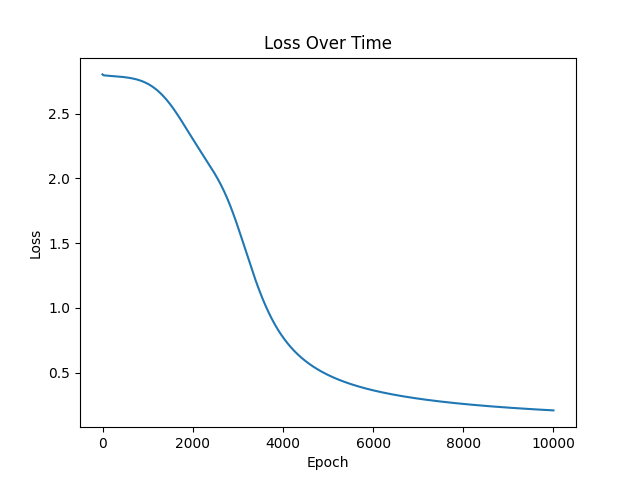
\includegraphics[width=0.5\linewidth]{image.png}
\end{center}
\end{document}
